\documentclass[12pt]{article}

\title{Initial conditions}
\author{Jan Medlock et al.}

\usepackage{microtype}
\usepackage{tikz}
\usepackage{hyperref}
\hypersetup{breaklinks}
\hypersetup{pdfborder=0 0 0}
\usepackage{natbib}
\usepackage{hypernat}
\usepackage{amsmath}
\renewcommand{\vec}[1]{\mathbf{#1}}
\newcommand{\mat}[1]{\mathbf{#1}}
\DeclareMathOperator{\Prob}{Prob}
\DeclareMathOperator{\diag}{diag}
\newcommand{\md}{\mathrm{d}}
\newcommand{\me}{\mathrm{e}}
\newcommand{\mT}{\mathrm{T}}
\setcounter{MaxMatrixCols}{12}


\begin{document}

\maketitle

\section{Model}

We simplified the larger problem by using
\begin{itemize}
\item the birth hazard that is constant in time, and
\item the hazard for antibody gain that is constant in time.
\end{itemize}
We found the equilibrium of this problem by iteratively solving for
the fixed point of the hazard of infection, $h_{\text{infection}}$,
and the fraction of newborns with maternal immunity,
$\phi_{\text{maternal immunity}}$. With given values of
$h_{\text{infection}}$ and $\phi_{\text{maternal immunity}}$, we
solved a linear-algebra problem for the equilibrium
probability densities as a function of model compartment, age, and
duration in the current compartment
(\autoref{model_diagram}), i.e.
\begin{subequations}
  \begin{align}
    P_{\mathrm{M}}(a)
    &= \Prob\{\text{in compartment $\mathrm{M}$ at age $a$}\},\\
    P_{\mathrm{S}}(a)
    &= \Prob\{\text{in compartment $\mathrm{S}$ at age $a$}\},\\
    p_{\mathrm{E}}(a, r)
    &= \Prob\{\text{in compartment $\mathrm{E}$ at age $a$ and
      duration $r$}\},\\
    p_{\mathrm{I}}(a, r)
    &= \Prob\{\text{in compartment $\mathrm{I}$ at age $a$ and
      duration $r$}\},\\
    p_{\mathrm{C}}(a, r)
    &= \Prob\{\text{in compartment $\mathrm{C}$ at age $a$ and
      duration $r$}\},\\
    P_{\mathrm{R}}(a)
    &= \Prob\{\text{in compartment $\mathrm{R}$ at age $a$}\},\\
    P_{\mathrm{L}}(a)
    &= \Prob\{\text{in compartment $\mathrm{L}$ at age $a$}\},
  \end{align}
\end{subequations}
for $a \geq 0$ and $0 \leq r \leq a$.
These $P_X(a)$ and $p_X(a, r)$ were then used to iteratively update
$h_{\text{infection}}$ and $\phi_{\text{maternal immunity}}$. Finally,
the equilibrium densities $P_X(a)$ were found at this fixed point.

\begin{figure}
  \begin{center}
    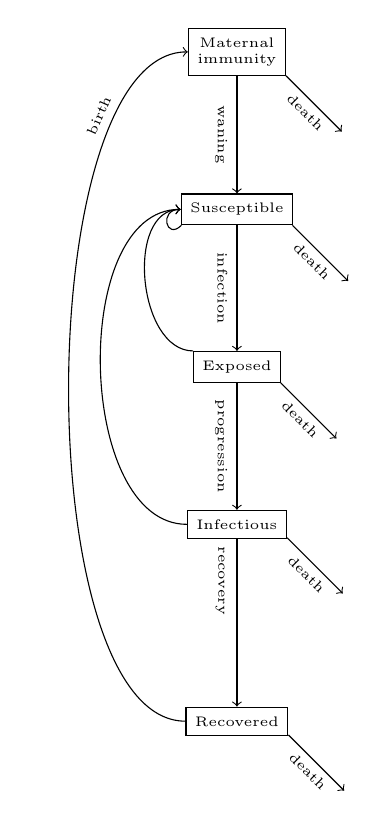
\begin{tikzpicture}[compartment/.style = {rectangle, draw}, font=\fontsize{5pt}{6}\selectfont]
  % Compartments.
  \node at (0, 11) [compartment, align=center, name=MaternalImmunity] {Maternal\\immunity};
  \node at (0, 9) [compartment, name=Susceptible] {Susceptible};
  \node at (0, 7) [compartment, name=Exposed] {Exposed};
  \node at (0, 5) [compartment, name=Infectious] {Infectious};
  \node at (0, 2.5) [compartment, name=Recovered] {Recovered};

  % Location for branch from Infectious to Chronic and Recovered.
  \coordinate (recovery) at (0, 3.75);

  % Infection-related processes.
  \draw [->] (MaternalImmunity)
             to node [rotate=-90, below] {waning}
             (Susceptible);
  \draw [->] (Susceptible)
             to node [rotate=-90, below] {infection}
             (Exposed);
  \draw [->] (Exposed)
             to node [rotate=-90, below] {progression}
             (Infectious);
  \draw [  ] (Infectious)
             to node [rotate=-90, below, yshift=-1pt] {recovery}
             (recovery);
  \draw [->] (recovery)
             to node [] {}
             (Recovered.90);

  % Births
  \draw [->] (Susceptible.196)
             to [out=225, in=180, looseness=3.5] node [] {}
             (Susceptible.180);
  \draw [->] (Exposed.160)
             to [out=180, in=180] node [] {}
             (Susceptible.180);
  \draw [->] (Infectious.180)
             to [out=180, in=180, looseness=0.9] node [sloped, above, pos=0.85] {}
             (Susceptible.180);
  \draw [->] (Recovered.180)
             to [out=180, in=180, looseness=0.6] node [sloped, above, pos=0.8] {birth}
             (MaternalImmunity.180);

  % Deaths
  \draw [->] (MaternalImmunity.334)
             to node [sloped, below, yshift=1pt] {death}
             +(315: 1);
  \draw [->] (Susceptible.344)
             to node [sloped, below, yshift=1pt] {death}
             +(315: 1);
  \draw [->] (Exposed.340)
             to node [sloped, below, yshift=1pt] {death}
             +(315: 1);
  \draw [->] (Infectious.345)
             to node [sloped, below, yshift=1pt] {death}
             +(315: 1);
  \draw [->] (Recovered.345)
             to node [sloped, below, yshift=1pt] {death}
             +(315: 1);
\end{tikzpicture}

%%% Local Variables:
%%% mode: latex
%%% TeX-master: "diagram_standalone"
%%% End:

  \end{center}
  \caption{Model diagram.}
  \label{model_diagram}
\end{figure}

For $a > 0$ and $0 < r \leq a$, the equilibrium probability densities
satisfy
\begin{subequations}
  \begin{align}
    P_{\mathrm{M}}(0)
    &= \phi_{\text{maternal immunity}},
    \\
    \frac{\md P_{\mathrm{M}}}{\md a}
    &= - \left[h_{\text{waning}}(a) + h_{\text{death}}(a)\right]
      P_{\mathrm{M}}(a),
    \displaybreak[0]\\
    P_{\mathrm{S}}(0)
    &= 1 - \phi_{\text{maternal immunity}},
    \\
    \frac{\md P_{\mathrm{S}}}{\md a}
    &= h_{\text{waning}}(a) P_{\mathrm{M}}(a)
      - \left[h_{\text{infection}} + h_{\text{death}}(a)\right]
      P_{\mathrm{S}}(a),
    \displaybreak[0]\\
    p_{\mathrm{E}}(0, 0) &= 0,
    \\
    p_{\mathrm{E}}(a, 0)
    &= h_{\text{infection}}
      \left[P_{\mathrm{S}}(a) + P_{\mathrm{L}}(a)\right],
    \\
    \left(\frac{\partial}{\partial a}
    + \frac{\partial}{\partial r}\right)
    p_{\mathrm{E}}
    &= - \left[h_{\text{progression}}(r) + h_{\text{death}}(a)\right]
      p_{\mathrm{E}}(a, r),
    \displaybreak[0]\\
    p_{\mathrm{I}}(0, 0) &= 0,
    \\
    p_{\mathrm{I}}(a, 0)
    &= \int_0^a h_{\text{progression}}(r)
      p_{\mathrm{E}}(a, r) \md r,
    \\
    \left(\frac{\partial}{\partial a}
    + \frac{\partial}{\partial r}\right)
    p_{\mathrm{I}}
    &= - \left[h_{\text{recovery}}(r) + h_{\text{death}}(a)\right]
      p_{\mathrm{I}}(a, r),
    \displaybreak[0]\\
    p_{\mathrm{C}}(0, 0) &= 0,
    \\
    p_{\mathrm{C}}(a, 0)
    &= p_{\text{chronicity}}
      \int_0^a h_{\text{recovery}}(r) p_{\mathrm{I}}(a, r) \md r,
    \\
    \left(\frac{\partial}{\partial a}
    + \frac{\partial}{\partial r}\right)
    p_{\mathrm{C}}
    &= - \left[h_{\text{chronic recovery}}(r) + h_{\text{death}}(a)\right]
      p_{\mathrm{C}}(a, r),
    \displaybreak[0]\\
    P_{\mathrm{R}}(0) &= 0,
    \\
    \begin{split}
      \frac{\md P_{\mathrm{R}}}{\md a} &=
      \left(1 - p_{\text{chronicity}}\right)
      \int_0^a h_{\text{recovery}}(r) p_{\mathrm{I}}(a, r) \md r
      \\ & \quad {}
      + \int_0^a h_{\text{chronic recovery}}(r) p_{\mathrm{C}}(a, r) \md r
      \\ & \quad {}
      + h_{\text{antibody gain}} P_{\mathrm{L}}(a)
      \\ & \quad {}
      - \left[h_{\text{antibody loss}} + h_{\text{death}}(a)\right]
      P_{\mathrm{R}}(a),
    \end{split}
    \displaybreak[0]\\
    P_{\mathrm{L}}(0) &= 0,
    \\
    \begin{split}
      \frac{\md P_{\mathrm{L}}}{\md a} &=
      h_{\text{antibody loss}} P_{\mathrm{R}}(a)
      \\ & \quad {}
      - \left[h_{\text{antibody gain}} + h_{\text{infection}}
        + h_{\text{death}}(a)\right]
      P_{\mathrm{L}}(a),
    \end{split}
  \end{align}
\end{subequations}
with
\begin{subequations}
  \begin{align}
    P_{\mathrm{E}}(a) &= \int_0^a p_{\mathrm{E}}(a, r) \md r,
    \displaybreak[0]\\
    P_{\mathrm{I}}(a) &= \int_0^a p_{\mathrm{I}}(a, r) \md r,
    \displaybreak[0]\\
    P_{\mathrm{C}}(a) &= \int_0^a p_{\mathrm{C}}(a, r) \md r.
  \end{align}
\end{subequations}

The infection hazard is
\begin{equation}
  h_{\text{infection}} =
  \int_0^{+\infty} N
  \left[
    \beta_{\text{infectious}} P_{\mathrm{I}}(a)
    + \beta_{\text{chronic}} P_{\mathrm{C}}(a)
  \right]
  \md a
\end{equation}
and the proportion of births that have maternal immunity is
\begin{equation}
  \phi_{\text{maternal immunity}}
  = \frac{
    \int_0^{+\infty} h_{\text{birth}}(a)
    \left[
      P_{\mathrm{M}}(a) + P_{\mathrm{C}}(a) + P_{\mathrm{R}}(a)
    \right]
    \md a
  }{
    \int_0^{+\infty} h_{\text{birth}}(a) P(a) \md a
  },
\end{equation}
where
\begin{equation}
  P(a)
  = P_{\mathrm{M}}(a) + P_{\mathrm{S}}(a) + P_{\mathrm{E}}(a)
  + P_{\mathrm{I}}(a) + P_{\mathrm{C}}(a) + P_{\mathrm{R}}(a)
  + P_{\mathrm{L}}(a),
\end{equation}
and $N$ is the population size.


\subsection{Analysis}

Integrating the PDEs along the characteristics $r = a - a_0$ gives
\begin{subequations}
  \begin{align}
    P_{\mathrm{M}}(0)
    &= \phi_{\text{maternal immunity}},
    \\
    \frac{\md P_{\mathrm{M}}}{\md a}
    &= - \left[h_{\text{waning}}(a) + h_{\text{death}}(a)\right]
      P_{\mathrm{M}}(a),
    \displaybreak[0]\\
    P_{\mathrm{S}}(0)
    &= 1 - \phi_{\text{maternal immunity}},
    \\
    \frac{\md P_{\mathrm{S}}}{\md a}
    &= h_{\text{waning}}(a) P_{\mathrm{M}}(a)
      - \left[h_{\text{infection}}  + h_{\text{death}}(a)\right]
      P_{\mathrm{S}}(a),
    \displaybreak[0]\\
    p_{\mathrm{E}}(0, 0) &= 0,
    \\
    p_{\mathrm{E}}(a, 0)
    &= h_{\text{infection}}
      \left[P_{\mathrm{S}}(a) + P_{\mathrm{L}}(a)\right],
    \\
    p_{\mathrm{E}}(a, r)
    &= S_{\text{progression}}(r)
      \frac{S_{\text{death}}(a)}{S_{\text{death}}(a - r)}
      p_{\mathrm{E}}(a - r, 0),
    \displaybreak[0]\\
    p_{\mathrm{I}}(0, 0) &= 0,
    \\
    p_{\mathrm{I}}(a, 0)
    &= \int_0^a
      p_{\text{progression}}(r)
      \frac{S_{\text{death}}(a)}{S_{\text{death}}(a - r)}
      p_{\mathrm{E}}(a - r, 0)
      \md r,
    \\
    p_{\mathrm{I}}(a, r)
    &= S_{\text{recovery}}(r)
      \frac{S_{\text{death}}(a)}{S_{\text{death}}(a - r)}
      p_{\mathrm{I}}(a - r, 0),
    \displaybreak[0]\\
    p_{\mathrm{C}}(0, 0) &= 0,
    \\
    p_{\mathrm{C}}(a, 0)
    &= p_{\text{chronicity}}
      \int_0^a
      p_{\text{recovery}}(r)
      \frac{S_{\text{death}}(a)}{S_{\text{death}}(a - r)}
      p_{\mathrm{I}}(a - r, 0)
      \md r,
    \\
    p_{\mathrm{C}}(a, r)
    &= S_{\text{chronic recovery}}(r)
      \frac{S_{\text{death}}(a)}{S_{\text{death}}(a - r)}
      p_{\mathrm{C}}(a - r, 0),
    \displaybreak[0]\\
    P_{\mathrm{R}}(0) &= 0,
    \\
    \begin{split}
      \frac{\md P_{\mathrm{R}}}{\md a} &=
      \left(1 - p_{\text{chronicity}}\right)
      \int_0^a
      p_{\text{recovery}}(r)
      \frac{S_{\text{death}}(a)}{S_{\text{death}}(a - r)}
      p_{\mathrm{I}}(a - r, 0)
      \md r
      \\ & \quad {}
      + \int_0^a
      p_{\text{chronic recovery}}(r)
      \frac{S_{\text{death}}(a)}{S_{\text{death}}(a - r)}
      p_{\mathrm{C}}(a - r, 0)
      \md r
      \\ & \quad {}
      + h_{\text{antibody gain}} P_{\mathrm{L}}(a)
      \\ & \quad {}
      - \left[h_{\text{antibody loss}}  + h_{\text{death}}(a)\right]
      P_{\mathrm{R}}(a),
    \end{split}
    \displaybreak[0]\\
    P_{\mathrm{L}}(0) &= 0,
    \\
    \begin{split}
      \frac{\md P_{\mathrm{L}}}{\md a}
      &= h_{\text{antibody loss}} P_{\mathrm{R}}(a)
      \\ & \quad {}
      - \left[h_{\text{antibody gain}} + h_{\text{infection}}
        + h_{\text{death}}(a)\right]
      P_{\mathrm{L}}(a).
    \end{split}
  \end{align}
\end{subequations}

Using
\begin{subequations}
  \label{eq:integrals_over_r}
  \begin{align}
    P_{\mathrm{E}}(a)
    &= \int_0^a
      S_{\text{progression}}(a - a_0)
      \frac{S_{\text{death}}(a)}{S_{\text{death}}(a_0)}
      p_{\mathrm{E}}(a_0, 0)
      \md a_0,
    \displaybreak[0]\\
    P_{\mathrm{I}}(a)
    &= \int_0^a
      S_{\text{recovery}}(a - a_0)
      \frac{S_{\text{death}}(a)}{S_{\text{death}}(a_0)}
      p_{\mathrm{I}}(a_0, 0)
      \md a_0,
    \displaybreak[0]\\
    P_{\mathrm{C}}(a)
    &= \int_0^a
      S_{\text{chronic recovery}}(a - a_0)
      \frac{S_{\text{death}}(a)}{S_{\text{death}}(a_0)}
      p_{\mathrm{C}}(a_0, 0)
      \md a_0,
  \end{align}
\end{subequations}
gives
\begin{subequations}
  \label{eq:integrals_derivatives}
  \begin{align}
    \begin{split}
      \frac{\md P_{\mathrm{E}}}{\md a}
      &= h_{\text{infection}}
      \left[P_{\mathrm{S}}(a) + P_{\mathrm{L}}(a)\right]
      \\ & \quad {}
      - \int_0^a
      p_{\text{progression}}(r)
      \frac{S_{\text{death}}(a)}{S_{\text{death}}(a - r)}
      p_{\mathrm{E}}(a - r, 0)
      \md r
      \\ & \quad {}
      - h_{\text{death}}(a) P_{\mathrm{E}}(a),
    \end{split}
    \displaybreak[0]\\
    \begin{split}
      \frac{\md P_{\mathrm{I}}}{\md a}
      &= \int_0^a
      p_{\text{progression}}(r)
      \frac{S_{\text{death}}(a)}{S_{\text{death}}(a - r)}
      p_{\mathrm{E}}(a - r, 0) \md r
      \\ & \quad {}
      - \int_0^a
      p_{\text{recovery}}(r)
      \frac{S_{\text{death}}(a)}{S_{\text{death}}(a - r)}
      p_{\mathrm{I}}(a - r, 0)
      \md r
      \\ & \quad {}
      - h_{\text{death}}(a) P_{\mathrm{I}}(a),
    \end{split}
    \displaybreak[0]\\
    \begin{split}
      \frac{\md P_{\mathrm{C}}}{\md a}
      &= p_{\text{chronicity}}
      \int_0^a
      p_{\text{recovery}}(r)
      \frac{S_{\text{death}}(a)}{S_{\text{death}}(a - r)}
      p_{\mathrm{I}}(a - r, 0)
      \md r
      \\ & \quad {}
      - \int_0^a
      p_{\text{chronic recovery}}(r)
      \frac{S_{\text{death}}(a)}{S_{\text{death}}(a - r)}
      p_{\mathrm{C}}(a - r, 0)
      \md r
      \\ & \quad {}
      - h_{\text{death}}(a) P_{\mathrm{C}}(a).
    \end{split}
  \end{align}
\end{subequations}
Then
\begin{subequations}
  \begin{align}
    \frac{\md P}{\md a}
    &= - h_{\text{death}}(a) P(a), \\
    P(0) &= 1,
  \end{align}
\end{subequations}
so that
\begin{equation}
  P(a) = S_{\text{death}}(a).
\end{equation}

The constant-time birth hazard
(i.e.~$c_{\mathrm{v}} = 0$)
\begin{equation}
  h_{\text{birth}}(a) =
  \begin{cases}
    0 & \text{if $a < 4$}, \\
    \mu & \text{if $a \geq 4$},
  \end{cases}
\end{equation}
with
\begin{equation}
  \mu =
  \left[
    \int_4^{+\infty} S_{\text{death}}(a) \md a
  \right]^{-1},
\end{equation}
gives
\begin{equation}
  \int_0^{+\infty} h_{\text{birth}}(a) P(a) \md a
  = \int_0^{+\infty} h_{\text{birth}}(a) S_{\text{death}}(a) \md a
  = 1
  = P(0),
\end{equation}
so that the population size is constant, i.e.~zero growth rate.


\section{Numerical method}

To compute the probability densities, we used the Crank--Nicolson
method on characteristics and the composite trapezoid rule for the
integrals \citep{milner_1992}.  Given the age step $\Delta a$,
for $i \in \{0, 1, 2, \ldots, I - 1\}$ and
$j \in \{0, 1, 2, \ldots, i\}$, let $a^i = i \Delta a$, $r^j = j
\Delta a$, $P_X^i \approx P_X(a^i)$, and
$p_X^i \approx p_X(a^i, 0)$.
For each $i \in \{1, 2, \ldots, I - 1\}$, using the
Crank--Nicolson method on characteristics gives
\begin{subequations}
  \label{eq:numerical_method}
  \begin{align}
    P_{\mathrm{M}}^0
    &= \phi_{\text{maternal immunity}},
    \\
    \frac{P_{\mathrm{M}}^i - P_{\mathrm{M}}^{i - 1}}{\Delta a}
    &= - \left[
      h_{\text{waning}}(a^{i - 1 / 2})
      + h_{\text{death}}(a^{i - 1 / 2})
      \right]
      \frac{P_{\mathrm{M}}^i + P_{\mathrm{M}}^{i - 1}}{2},
    \displaybreak[0]\\
    P_{\mathrm{S}}^0
    &= 1 - \phi_{\text{maternal immunity}},
    \\
    \begin{split}
      \frac{P_{\mathrm{S}}^i - P_{\mathrm{S}}^{i - 1}}{\Delta a}
      &= h_{\text{waning}}(a^{i - 1 / 2})
      \frac{P_{\mathrm{M}}^i + P_{\mathrm{M}}^{i - 1}}{2}
      \\ & \quad {}
      - \left[
        h_{\text{infection}}
        + h_{\text{death}}(a^{i - 1 / 2})
      \right]
      \frac{P_{\mathrm{S}}^i + P_{\mathrm{S}}^{i - 1}}{2},
    \end{split}
    \displaybreak[0]\\
    p_{\mathrm{E}}^0 &= 0,
    \\
    p_{\mathrm{E}}^i
    &= h_{\text{infection}} \left(
      \frac{P_{\mathrm{S}}^i + P_{\mathrm{S}}^{i - 1}}{2}
      + \frac{P_{\mathrm{L}}^i + P_{\mathrm{L}}^{i - 1}}{2}
      \right),
    \displaybreak[0]\\
    p_{\mathrm{I}}^0 &= 0,
    \\
    p_{\mathrm{I}}^i
    &= \sum_{j = 0}^i  % or start at j = 1?
      p_{\text{progression}}(r^j)
      \frac{S_{\text{death}}(a^i)}{S_{\text{death}}(a^{i - j})}
      p_{\mathrm{E}}^{i - j}
      \Delta a,
    \displaybreak[0]\\
    p_{\mathrm{C}}^0 &= 0,
    \\
    p_{\mathrm{C}}^i
    &= p_{\text{chronicity}}
      \sum_{j = 0}^i % or start at j = 1?
      p_{\text{recovery}}(r^j)
      \frac{S_{\text{death}}(a^i)}{S_{\text{death}}(a^{i - j})}
      p_{\mathrm{I}}^{i - j}
      \Delta a,
    \displaybreak[0]\\
    P_{\mathrm{R}}^0 &= 0,
    \\
    \begin{split}
      \frac{P_{\mathrm{R}}^i - P_{\mathrm{R}}^{i - 1}}{\Delta a}
      &= \left(1 - p_{\text{chronicity}}\right)
      \sum_{j = 0}^i  % or start at j = 1?
      p_{\text{recovery}}(r^j)
      \frac{S_{\text{death}}(a^i)}{S_{\text{death}}(a^{i - j})}
      p_{\mathrm{I}}^{i - j}
      \Delta a
      \\ & \quad {}
      + \sum_{j = 0}^i % or start at j = 1?
      p_{\text{chronic recovery}}(r^j)
      \frac{S_{\text{death}}(a^i)}{S_{\text{death}}(a^{i - j})}
      p_{\mathrm{C}}^{i - j}
      \Delta a
      \\ & \quad {}
      + h_{\text{antibody gain}}
      \frac{P_{\mathrm{L}}^i + P_{\mathrm{L}}^{i - 1}}{2}
      \\ & \quad {}
      - \left[
        h_{\text{antibody loss}} + h_{\text{death}}(a^{i - 1 / 2})
      \right]
      \frac{P_{\mathrm{R}}^i + P_{\mathrm{R}}^{i - 1}}{2},
    \end{split}
    \displaybreak[0]\\
    P_{\mathrm{L}}^0 &= 0,
    \\
    \begin{split}
      \frac{P_{\mathrm{L}}^i - P_{\mathrm{L}}^{i - 1}}{\Delta a}
      &= h_{\text{antibody loss}}
      \frac{P_{\mathrm{R}}^i + P_{\mathrm{R}}^{i - 1}}{2}
      \\ & \quad {}
      - \left[
        h_{\text{antibody gain}} + h_{\text{infection}}
        + h_{\text{death}}(a^{i - 1 / 2})
      \right]
      \frac{P_{\mathrm{L}}^i + P_{\mathrm{L}}^{i - 1}}{2},
    \end{split}
  \end{align}
\end{subequations}
with
\begin{subequations}
  \label{eq:sums_over_r}
  \begin{align}
    P_{\mathrm{E}}^i
    &= \sum_{j = 0}^i
      S_{\text{progression}}(r^j)
      \frac{S_{\text{death}}(a^i)}{S_{\text{death}}(a^{i - j})}
      p_{\mathrm{E}}^{i - j}
      \Delta a,
    \displaybreak[0]\\
    P_{\mathrm{I}}^i
    &= \sum_{j = 0}^i
      S_{\text{recovery}}(r^j)
      \frac{S_{\text{death}}(a^i)}{S_{\text{death}}(a^{i - j})}
      p_{\mathrm{I}}^{i - j}
      \Delta a,
    \displaybreak[0]\\
    P_{\mathrm{C}}^i
    &= \sum_{j = 0}^i
      S_{\text{chronic recovery}}(r^j)
      \frac{S_{\text{death}}(a^i)}{S_{\text{death}}(a^{i - j})}
      p_{\mathrm{C}}^{i - j}
      \Delta a.
  \end{align}
\end{subequations}

The infection hazard is
\begin{equation}
  h_{\text{infection}}
  = \sum_{i = 0}^{I - 1} N
  \left(
    \beta_{\text{infectious}} P_{\mathrm{I}}^i
    + \beta_{\text{chronic}} P_{\mathrm{C}}^i
  \right)
  \Delta a,
\end{equation}
and the proportion of births that have maternal immunity is
\begin{equation}
  \phi_{\text{maternal immunity}}
  = \frac{
    \sum_{i = 0}^{I - 1}
    h_{\text{birth}}(a^i) \left(
      P_{\mathrm{M}}^i + P_{\mathrm{C}}^i + P_{\mathrm{R}}^i
    \right)
    \Delta a
  }{
    \sum_{i = 0}^{I - 1} h_{\text{birth}}(a^i) P^i \Delta a
  },
\end{equation}
where
\begin{equation}
  P^i =  P_{\mathrm{M}}^i + P_{\mathrm{S}}^i + P_{\mathrm{E}}^i
  + P_{\mathrm{I}}^i + P_{\mathrm{C}}^i + P_{\mathrm{R}}^i + P_{\mathrm{L}}^i,
\end{equation}
and $N$ is the population size.

\subsection{Analysis}

The differences of the sums \eqref{eq:sums_over_r} are
\begin{equation}
  \label{eq:sums_differences}
  \begin{split}
    \frac{P_X^i - P_X^{i - 1}}{\Delta a}
    &=
    \sum_{j = 0}^i S_{Y_X}(r^j)
    \frac{S_{\text{death}}(a^i)}{S_{\text{death}}(a^{i - j})}
    p_X^{i - j}
    \\ & \quad {}
    - \sum_{j = 0}^{i - 1} S_{Y_X}(r^j)
    \frac{S_{\text{death}}(a^{i - 1})}{S_{\text{death}}(a^{i - 1 - j})}
    p_X^{i - 1 - j}
    \\
    &= p_X^i
    + \sum_{j = 1}^i S_{Y_X}(r^j)
    \frac{S_{\text{death}}(a^i)}{S_{\text{death}}(a^{i - j})}
    p_X^{i - j}
    \\ & \quad {}
    - \sum_{j = 1}^i S_{Y_X}(r^{j - 1})
    \frac{S_{\text{death}}(a^{i - 1})}{S_{\text{death}}(a^{i - j})}
    p_X^{i - j}
    \\
    &= p_X^i
    - \sum_{j = 1}^i
    \left[
      S_{Y_X}(r^{j - 1})
      - S_{Y_X}(r^j)
    \right]
    \frac{S_{\text{death}}(a^i)}{S_{\text{death}}(a^{i - j})}
    p_X^{i - j}
    \\ & \quad {}
    - \sum_{j = 1}^i S_{Y_X}(r^{j - 1})
    \frac{S_{\text{death}}(a^{i - 1}) - S_{\text{death}}(a^i)}
    {S_{\text{death}}(a^{i - j})}
    p_X^{i - j}
    \\
    &= p_X^i
    - \sum_{j = 1}^i p_{Y_X}(r^j)
    \frac{S_{\text{death}}(a^i)}{S_{\text{death}}(a^{i - j})}
    p_X^{i - j} \Delta a
    \\ & \quad {}
    - \frac{S_{\text{death}}(a^{i - 1}) - S_{\text{death}}(a^i)}
    {S_{\text{death}}(a^{i - 1})}
    \sum_{j = 0}^{i - 1} S_{Y_X}(r^j)
    \frac{S_{\text{death}}(a^{i - 1})}{S_{\text{death}}(a^{i - 1 - j})}
    p_X^{i - 1 - j}
    \\
    &= p_X^i
    - \sum_{j = 0}^i p_{Y_X}(r^j)
    \frac{S_{\text{death}}(a^i)}{S_{\text{death}}(a^{i - j})}
    p_X^{i - j} \Delta a
    \\ & \quad {}
    + p_{Y_X}(0) p_X^i \Delta a
    - \frac{S_{\text{death}}(a^{i - 1}) - S_{\text{death}}(a^i)}
    {S_{\text{death}}(a^{i - 1})}
    \frac{P_X^{i - 1}}{\Delta a}
    \\
    &= p_X^i
    - \sum_{j = 0}^i p_{Y_X}(r^j)
    \frac{S_{\text{death}}(a^i)}{S_{\text{death}}(a^{i - j})}
    p_X^{i - j} \Delta a
    - h_{\text{death}}(a^{i - 1 / 2})
    \frac{P_X^i + P_X^{i - 1}}{2}
    \\ & \quad {}
    + p_{Y_X}(0) p_X^i \Delta a
    - \frac{S_{\text{death}}(a^{i - 1}) - S_{\text{death}}(a^i)}
    {S_{\text{death}}(a^{i - 1})}
    \frac{P_X^{i - 1}}{\Delta a}
    + h_{\text{death}}(a^{i - 1 / 2})
    \frac{P_X^i + P_X^{i - 1}}{2},
  \end{split}
\end{equation}
%
\textbf{TODO: \eqref{eq:sums_differences} should look like
  \eqref{eq:integrals_derivatives}. In particular, the last 3 terms should
  all cancel each other.}
%
for
\begin{equation}
  X \in \{\mathrm{E}, \mathrm{I}, \mathrm{C}\},
\end{equation}
and
\begin{equation}
  \begin{split}
    Y_{\mathrm{E}} &= \text{progression},
    \\
    Y_{\mathrm{I}} &= \text{recovery},
    \\
    Y_{\mathrm{C}} &= \text{chronic recovery}.
  \end{split}
\end{equation}

Then
\begin{subequations}
  \begin{align}
    P^0 &= 1,
    \displaybreak[0]\\
    \begin{split}
      \frac{P^i - P^{i - 1}}{\Delta a}
      &= - h_{\text{death}}(a^{i - 1 / 2})
      \frac{P^i + P^{i - 1}}{2}
      \\ & \quad {}
      % or start sum in (14h) at j = 1?
      + p_{\text{progression}}(0) p_{\mathrm{E}}^i \Delta a
      % or start sums in (14j) & (14l) at j = 1?
      + p_{\text{recovery}}(0) p_{\mathrm{I}}^i \Delta a
      % or start sum in (14l) at j = 1?
      + p_{\text{chronic recovery}}(0) p_{\mathrm{C}}^i \Delta a
      \\ & \quad {}
      + h_{\text{death}}(a^{i - 1 / 2})
      \left(
        \frac{P_{\mathrm{E}}^i + P_{\mathrm{E}}^{i - 1}}{2}
        + \frac{P_{\mathrm{I}}^i + P_{\mathrm{I}}^{i - 1}}{2}
        + \frac{P_{\mathrm{C}}^i + P_{\mathrm{C}}^{i - 1}}{2}
      \right)
      \\ & \quad {}
      - \frac{S_{\text{death}}(a^{i - 1}) - S_{\text{death}}(a^i)}
      {S_{\text{death}}(a^{i - 1})}
      \left(P_{\mathrm{E}}^{i - 1} + P_{\mathrm{I}}^{i - 1}
        + P_{\mathrm{C}}^{i - 1}\right)
      \frac{1}{\Delta a}
      \\
      &= - h_{\text{death}}(a^{i - 1 / 2})
      \frac{P^i + P^{i - 1}}{2}
      \\ & \quad {}
      % or start sum in (14h) at j = 1?
      + p_{\text{progression}}(0) p_{\mathrm{E}}^i \Delta a
      % or start sums in (14j) & (14l) at j = 1?
      + p_{\text{recovery}}(0) p_{\mathrm{I}}^i \Delta a
      % or start sum in (14l) at j = 1?
      + p_{\text{chronic recovery}}(0) p_{\mathrm{C}}^i \Delta a
      \\ & \quad {}
      + h_{\text{death}}(a^{i - 1 / 2})
      \left(
        \frac{P_{\mathrm{E}}^i + P_{\mathrm{E}}^{i - 1}}{2}
        + \frac{P_{\mathrm{I}}^i + P_{\mathrm{I}}^{i - 1}}{2}
        + \frac{P_{\mathrm{C}}^i + P_{\mathrm{C}}^{i - 1}}{2}
      \right)
      \\ & \quad {}
      - \frac{h_{\text{death}}(a^{i - 1 / 2})}
      {1 + h_{\text{death}}(a^{i - 1 / 2}) \Delta a / 2}
      \left(
        P_{\mathrm{E}}^{i - 1} + P_{\mathrm{I}}^{i - 1}
        + P_{\mathrm{C}}^{i - 1}
      \right)
      \\
      &= - h_{\text{death}}(a^{i - 1 / 2})
      \frac{P^i + P^{i - 1}}{2}
      \\ & \quad {}
      % or start sum in (14h) at j = 1?
      + p_{\text{progression}}(0) p_{\mathrm{E}}^i \Delta a
      % or start sums in (14j) & (14l) at j = 1?
      + p_{\text{recovery}}(0) p_{\mathrm{I}}^i \Delta a
      % or start sum in (14l) at j = 1?
      + p_{\text{chronic recovery}}(0) p_{\mathrm{C}}^i \Delta a
      \\ & \quad {}
      + \frac{1}{2} h_{\text{death}}(a^{i - 1 / 2})
      \left[
        \left(P_{\mathrm{E}}^i
          + P_{\mathrm{I}}^i
          + P_{\mathrm{C}}^i
        \right)
        - \frac{1 - h_{\text{death}}(a^{i - 1 / 2}) \Delta a / 2}
        {1 + h_{\text{death}}(a^{i - 1 / 2}) \Delta a / 2}
        \left(
          P_{\mathrm{E}}^{i - 1}
          + P_{\mathrm{I}}^{i - 1}
          + P_{\mathrm{C}}^{i - 1}
        \right)
      \right]
      \\
      &= - h_{\text{death}}(a^{i - 1 / 2})
      \frac{P^i + P^{i - 1}}{2}
      \\ & \quad {}
      % or start sum in (14h) at j = 1?
      + p_{\text{progression}}(0) p_{\mathrm{E}}^i \Delta a
      % or start sums in (14j) & (14l) at j = 1?
      + p_{\text{recovery}}(0) p_{\mathrm{I}}^i \Delta a
      % or start sum in (14l) at j = 1?
      + p_{\text{chronic recovery}}(0) p_{\mathrm{C}}^i \Delta a
      \\ & \quad {}
      + \frac{1}{2} h_{\text{death}}(a^{i - 1 / 2})
      \left[
        \left(P_{\mathrm{E}}^i
          + P_{\mathrm{I}}^i
          + P_{\mathrm{C}}^i
        \right)
        - \frac{S_{\text{death}}(a^i)}{S_{\text{death}}(a^{i - 1})}
        \left(
          P_{\mathrm{E}}^{i - 1}
          + P_{\mathrm{I}}^{i - 1}
          + P_{\mathrm{C}}^{i - 1}
        \right)
      \right].
    \end{split}
  \end{align}
\end{subequations}
%
\textbf{TODO: All the terms after the top line should cancel each
  other. From \eqref{eq:discrete_total}, we have the Crank--Nicholson
  approximation of the survival in terms of the hazard}
\begin{displaymath}
  S_{\text{death}}(a^i)
  = \prod_{j = 1}^i \frac{
    1 - h_{\text{death}}(a^{j - 1 / 2}) \Delta a / 2
  }{
    1 + h_{\text{death}}(a^{j - 1 / 2}) \Delta a / 2
  }.
\end{displaymath}
\textbf{This gives}
\begin{displaymath}
  \begin{split}
    \frac{
      S_{\text{death}}(a^{i - 1}) - S_{\text{death}}(a^i)
    }{
      S_{\text{death}}(a^{i - 1})
    }
    &= \frac{
      h_{\text{death}}(a^{i - 1 / 2}) \Delta a
    }{
      1 + h_{\text{death}}(a^{i - 1 / 2}) \Delta a / 2
    }.
  \end{split}
\end{displaymath}
%

Then
\begin{equation}
  \frac{P^i - P^{i - 1}}{\Delta a}
  = - h_{\text{death}}(a^{i - 1 / 2})
  \frac{P^i + P^{i - 1}}{2},
\end{equation}
so that
\begin{equation}
  \label{eq:discrete_total}
  \begin{split}
    P^i
    &= \frac{
      1 - h_{\text{death}}(a^{i - 1 / 2}) \Delta a / 2
    }{
      1 + h_{\text{death}}(a^{i - 1 / 2}) \Delta a / 2
    } P^{i - 1}
    \\
    &= \prod_{j = 1}^i \frac{
      1 - h_{\text{death}}(a^{j - 1 / 2}) \Delta a / 2
    }{
      1 + h_{\text{death}}(a^{j - 1 / 2}) \Delta a / 2
    }
    \\
    &= S_{\text{death}}(a^i).
  \end{split}
\end{equation}

The the constant-time birth hazard
(i.e.~$c_{\mathrm{v}} = 0$)
\begin{equation}
  h_{\text{birth}}(a) =
  \begin{cases}
    0 & \text{if $a < 4$}, \\
    \mu & \text{if $a \geq 4$},
  \end{cases}
\end{equation}
with
\begin{equation}
  \mu =
  \left[
    \sum_{a^i \geq 4}
    S_{\text{death}}(a^i)
    \Delta a
  \right]^{-1},
\end{equation}
gives
\begin{equation}
  \sum_{i = 0}^{I - 1}
  h_{\text{birth}}(a^i) P^i
  \Delta a
  = \sum_{i = 0}^{I - 1}
  h_{\text{birth}}(a^i) S_{\text{death}}(a^i)
  \Delta a
  = 1 = P^0,
\end{equation}
so that the population size is constant, i.e.~zero growth rate.


\section{Implementation}

The numerical scheme can be written as
\begin{subequations}
\begin{align}
  P_{\mathrm{M}}^0 &= \phi_{\text{maternal immunity}},
  \displaybreak[0]\\
  \begin{split}
    - \left\{1
      - \left[h_{\text{waning}}(a^{i - 1 / 2})
        + h_{\text{death}}(a^{i - 1 / 2})\right]
      \frac{\Delta a}{2}\right\}
    P_{\mathrm{M}}^{i - 1}
    \\ {}
    + \left\{1
      + \left[h_{\text{waning}}(a^{i - 1 / 2})
        + h_{\text{death}}(a^{i - 1 / 2})\right]
      \frac{\Delta a}{2}\right\}
    P_{\mathrm{M}}^i
    &= 0,
  \end{split}
  \displaybreak[0]\\
  P_{\mathrm{S}}^0 &= 1 - \phi_{\text{maternal immunity}},
  \displaybreak[0]\\
  \begin{split}
    - h_{\text{waning}}(a^{i - 1 / 2}) \frac{\Delta a}{2}
    P_{\mathrm{M}}^{i - 1}
    - h_{\text{waning}}(a^{i - 1 / 2}) \frac{\Delta a}{2}
    P_{\mathrm{M}}^i
    \\ {}
    - \left\{1
      - \left[h_{\text{infection}}
        + h_{\text{death}}(a^{i - 1 / 2})\right]
      \frac{\Delta a}{2}\right\}
    P_{\mathrm{S}}^{i - 1}
    \\ {}
    + \left\{1
      + \left[h_{\text{infection}}
        + h_{\text{death}}(a^{i - 1 / 2})\right]
        \frac{\Delta a}{2}\right\}
    P_{\mathrm{S}}^i
    &= 0,
  \end{split}
  \displaybreak[0]\\
  p_{\mathrm{E}}^0 &= 0,
  \\
  \begin{split}
    - \frac{h_{\text{infection}}}{2} P_{\mathrm{S}}^{i - 1}
    - \frac{h_{\text{infection}}}{2} P_{\mathrm{S}}^i
    \\ {}
    + p_{\mathrm{E}}^i
    \\ {}
    - \frac{h_{\text{infection}}}{2} P_{\mathrm{L}}^{i - 1}
    - \frac{h_{\text{infection}}}{2} P_{\mathrm{L}}^i
    &= 0,
  \end{split}
  \displaybreak[0]\\
  p_{\mathrm{I}}^0 &= 0,
  \\
  - \sum_{j = 0}^i p_{\text{progression}}(r^{i - j})
  \frac{S_{\text{death}}(a^i)}{S_{\text{death}}(a^j)}
  \Delta a
  p_{\mathrm{E}}^j
  + p_{\mathrm{I}}^i
  &= 0,
  \displaybreak[0]\\
  p_{\mathrm{C}}^0 &= 0,
  \\
  - \sum_{j = 0}^i
  p_{\text{chronicity}} p_{\text{recovery}}(r^{i - j})
  \frac{S_{\text{death}}(a^i)}{S_{\text{death}}(a^j)}
  \Delta a
  p_{\mathrm{I}}^j
  + p_{\mathrm{C}}^i
  &= 0,
  \displaybreak[0]\\
  P_{\mathrm{R}}^0 &= 0,
  \\
  \begin{split}
    - \sum_{j = 0}^i
    \left(1 - p_{\text{chronicity}}\right)
    p_{\text{recovery}}(r^{i - j})
    \frac{S_{\text{death}}(a^i)}{S_{\text{death}}(a^j)}
    \Delta a
    p_{\mathrm{I}}^j
    \\ {}
    - \sum_{j = 0}^i
    p_{\text{chronic recovery}}(r^{i - j})
    \frac{S_{\text{death}}(a^i)}{S_{\text{death}}(a^j)}
    \Delta a
    p_{\mathrm{C}}^j
    \\ {}
    - \left\{1
      - \left[h_{\text{antibody loss}}
        + h_{\text{death}}(a^{i - 1 / 2})
      \right]
      \frac{\Delta a}{2}\right\}
    P_{\mathrm{R}}^{i - 1}
    \\ {}
    + \left\{1
      + \left[h_{\text{antibody loss}}
        + h_{\text{death}}(a^{i - 1 / 2})\right]
      \frac{\Delta a}{2}\right\}
    P_{\mathrm{R}}^i
    \\ {}
    - h_{\text{antibody gain}} \frac{\Delta a}{2}
    P_{\mathrm{L}}^{i - 1}
    - h_{\text{antibody gain}} \frac{\Delta a}{2}
    P_{\mathrm{L}}^i
    &= 0,
  \end{split}
  \displaybreak[0]\\
  P_{\mathrm{L}}^0 &= 0,
  \\
  \begin{split}
    - h_{\text{antibody loss}} \frac{\Delta a}{2}
    P_{\mathrm{R}}^{i - 1}
    - h_{\text{antibody loss}} \frac{\Delta a}{2}
    P_{\mathrm{R}}^i
    \\ {}
    - \left\{1
      - \left[h_{\text{antibody gain}}
        + h_{\text{infection}}
        + h_{\text{death}}(a^{i - 1 / 2})
      \right]
      \frac{\Delta a}{2}\right\}
    P_{\mathrm{L}}^{i - 1}
    \\ {}
    + \left\{1
      + \left[h_{\text{antibody gain}}
        + h_{\text{infection}}
        + h_{\text{death}}(a^{i - 1 / 2})
        \right]
        \frac{\Delta a}{2}\right\}
    P_{\mathrm{L}}^i
    &= 0.
  \end{split}
\end{align}
\end{subequations}

Define the vectors
\begin{equation}
  \vec{x}_X =
  \begin{cases}
    \begin{pmatrix}
      P_X^0\\
      P_X^1\\
      \vdots\\
      P_X^{I - 1}
    \end{pmatrix}
    &
    \text{for $X \in
      \left\{\mathrm{M}, \mathrm{S}, \mathrm{R}, \mathrm{L}\right\}$},
    \\[4em]
    \begin{pmatrix}
      p_X^0\\
      p_X^1\\
      \vdots\\
      p_X^{I - 1}
    \end{pmatrix}
    &
    \text{for $X \in
      \left\{\mathrm{E}, \mathrm{I}, \mathrm{C}\right\}$},
  \end{cases}
\end{equation}
and let $\vec{x}$ be the $\vec{x}_X$'s stacked into a single vector,
\begin{equation}
  \vec{x} =
  \begin{pmatrix}
    \vec{x}_{\mathrm{M}}\\
    \vec{x}_{\mathrm{S}}\\
    \vec{x}_{\mathrm{E}}\\
    \vec{x}_{\mathrm{I}}\\
    \vec{x}_{\mathrm{C}}\\
    \vec{x}_{\mathrm{R}}\\
    \vec{x}_{\mathrm{L}}
  \end{pmatrix}.
\end{equation}

Define the birth matrix
\begin{equation}
  \mat{B} =
  \begin{bmatrix}
    \mat{B}_{\mathrm{M}} & \mat{0} & \mat{0} &
    \mat{0} & \mat{0} & \mat{0} & \mat{0}
    \\
    \mat{0} & \mat{B}_{\mathrm{S}} & \mat{0} &
    \mat{0} & \mat{0} & \mat{0} & \mat{0}
    \\
    \mat{0} & \mat{0} & \mat{0} & \mat{0} &
    \mat{0} & \mat{0} & \mat{0}
    \\
    \mat{0} & \mat{0} & \mat{0} & \mat{0} &
    \mat{0} & \mat{0} & \mat{0}
    \\
    \mat{0} & \mat{0} & \mat{0} & \mat{0} &
    \mat{0} & \mat{0} & \mat{0}
    \\
    \mat{0} & \mat{0} & \mat{0} & \mat{0} &
    \mat{0} & \mat{0} & \mat{0}
    \\
    \mat{0} & \mat{0} & \mat{0} & \mat{0} &
    \mat{0} & \mat{0} & \mat{0}
  \end{bmatrix},
\end{equation}
with blocks
\begin{equation}
  \mat{B}_{\mathrm{M}} = \mat{B}_{\mathrm{S}}
  =
  \begin{bmatrix}
    1 & 0 & \hdots & 0 \\
    0 & 0 & \hdots & 0 \\
    \vdots & \vdots & & \vdots \\
    0 & 0 & \hdots & 0
  \end{bmatrix}.
\end{equation}

Define the block diagonal matrix
\begin{align}
  \mat{D} &=
  \begin{bmatrix}
    \mat{D}_{\mathrm{M}} & \mat{0} & \mat{0} &
    \mat{0} & \mat{0} & \mat{0} & \mat{0}
    \\
    \mat{0} & \mat{D}_{\mathrm{S}} & \mat{0} &
    \mat{0} & \mat{0} & \mat{0} & \mat{0}
    \\
    \mat{0} & \mat{0} & \bar{\mat{D}}_{\mathrm{E}} &
    \mat{0} & \mat{0} & \mat{0} & \mat{0}
    \\
    \mat{0} & \mat{0} & \mat{0} &
    \bar{\mat{D}}_{\mathrm{I}} & \mat{0} & \mat{0} & \mat{0}
    \\
    \mat{0} & \mat{0} & \mat{0} & \mat{0} &
    \bar{\mat{D}}_{\mathrm{C}} & \mat{0} & \mat{0}
    \\
    \mat{0} & \mat{0} & \mat{0} & \mat{0} &
    \mat{0} & \mat{D}_{\mathrm{R}} & \mat{0}
    \\
    \mat{0} & \mat{0} & \mat{0} & \mat{0} &
    \mat{0} & \mat{0} & \mat{D}_{\mathrm{L}}
  \end{bmatrix},
\end{align}
with blocks
\begin{subequations}
  \begin{align}
    \mat{D}_X &=
    \begin{bmatrix}
      0 & 0 & 0 & \hdots & 0
      \\
      - 1 + d_X^1 & 1 + d_X^1 & 0 & \hdots & 0
      \\
      0 & - 1 + d_X^2 & 1 + d_X^2 & \ddots & \vdots
      \\
      \vdots & \ddots & \ddots & \ddots & 0
      \\
      0 & \hdots & 0 & - 1 + d_X^{I - 1} & 1 + d_X^{I - 1}
    \end{bmatrix},
    \\
    \bar{\mat{D}}_X &=
    \begin{bmatrix}
      1 & 0 & \hdots & 0 \\
      0 & 1 & \ddots & \vdots \\
      \vdots & \ddots & \ddots & 0 \\
      0 & \hdots & 0 & 1
    \end{bmatrix},
  \end{align}
\end{subequations}
where
\begin{subequations}
  \begin{align}
    d_{\mathrm{M}}^i
    &= \frac{1}{2} \left[h_{\text{waning}}(a^{i - 1 / 2})
      + h_{\text{death}}(a^{i - 1 / 2})\right]
      \Delta a,
    \\
    d_{\mathrm{S}}^i
    &= \frac{1}{2} \left[h_{\text{infection}}
      + h_{\text{death}}(a^{i - 1 / 2})\right]
      \Delta a,
    \\
    d_{\mathrm{R}}^i
    &= \frac{1}{2} \left[h_{\text{antibody loss}}
      + h_{\text{death}}(a^{i - 1 / 2})\right]
      \Delta a,
    \\
    d_{\mathrm{L}}^i
    &= \frac{1}{2} \left[h_{\text{antibody gain}}
      + h_{\text{infection}}
      + h_{\text{death}}(a^{i - 1 / 2})\right]
      \Delta a.
  \end{align}
\end{subequations}

Define the influx matrix
\begin{equation}
  \mat{F} =
  \begin{bmatrix}
    \mat{0} & \mat{0} & \mat{0} & \mat{0} &
    \mat{0} & \mat{0} & \mat{0}
    \\
    \mat{F}_{\mathrm{SM}} & \mat{0} & \mat{0} &
    \mat{0} & \mat{0} & \mat{0} & \mat{0}
    \\
    \mat{0} & \mat{F}_{\mathrm{ES}} & \mat{0} &
    \mat{0} & \mat{0} & \mat{0} & \mat{F}_{\mathrm{EL}}
    \\
    \mat{0} & \mat{0} & \bar{\mat{F}}_{\mathrm{IE}} &
    \mat{0} & \mat{0} & \mat{0} & \mat{0}
    \\
    \mat{0} & \mat{0} & \mat{0} & \bar{\mat{F}}_{\mathrm{CI}} &
    \mat{0} & \mat{0} & \mat{0}
    \\
    \mat{0} & \mat{0} & \mat{0} & \bar{\mat{F}}_{\mathrm{RI}} &
    \bar{\mat{F}}_{\mathrm{RC}} & \mat{0} & \mat{F}_{\mathrm{RL}}
    \\
    \mat{0} & \mat{0} & \mat{0} & \mat{0} &
    \mat{0} & \mat{F}_{\mathrm{LR}} & \mat{0}
  \end{bmatrix},
\end{equation}
with blocks
\begin{subequations}
  \begin{align}
    \mat{F}_{XY} &=
    \begin{bmatrix}
      0 & 0 & 0 & \hdots & 0
      \\
      f_{XY}^1 & f_{XY}^1 & 0 & \hdots & 0
      \\
      0 & f_{XY}^2 & f_{XY}^2 & \ddots & \vdots
      \\
      \vdots & \ddots & \ddots & \ddots & 0
      \\
      0 & \hdots & 0 & f_{XY}^{I - 1} &
      f_{XY}^{I - 1}
    \end{bmatrix},
    \displaybreak[0]\\
    \bar{\mat{F}}_{XY} &=
    \begin{bmatrix}
      % Maybe \bar{f}_{XY}^{0, 0} = 0 instead.
      \bar{f}_{XY}^{0, 0} & 0 & \hdots & 0
      \\
      \bar{f}_{XY}^{1, 0} & \bar{f}_{XY}^{1, 1} & \ddots & \vdots
      \\
      \vdots &  & \ddots & 0
      \\
      \bar{f}_{XY}^{I - 1, 0} & \bar{f}_{XY}^{I - 1, 1} & \hdots &
      \bar{f}_{XY}^{I - 1, I - 1}
    \end{bmatrix},
  \end{align}
\end{subequations}
where
\begin{subequations}
  \begin{align}
    f_{\mathrm{SM}}^i
    &= \frac{1}{2} h_{\text{waning}}(a^{i - 1 / 2}) \Delta a,
    \\
    f_{\mathrm{ES}}^i
    &= \frac{1}{2} h_{\text{infection}},
    \\
    f_{\mathrm{EL}}^i
    &= \frac{1}{2} h_{\text{infection}},
    \\
    f_{\mathrm{RL}}^i
    &= \frac{1}{2} h_{\text{antibody gain}} \Delta a,
    \\
    f_{\mathrm{LR}}^i
    &= \frac{1}{2} h_{\text{antibody loss}} \Delta a,
    \displaybreak[0]\\
    \bar{f}_{\mathrm{IE}}^{i, j}
    &= p_{\text{progression}}(r^{i - j})
      \frac{S_{\text{death}}(a^i)}{S_{\text{death}}(a^j)}
      \Delta a,
    \\
    \bar{f}_{\mathrm{CI}}^{i, j}
    &= p_{\text{chronicity}}
      p_{\text{recovery}}(r^{i - j})
      \frac{S_{\text{death}}(a^i)}{S_{\text{death}}(a^j)}
      \Delta a,
    \\
    \bar{f}_{\mathrm{RI}}^{i, j}
    &= (1 - p_{\text{chronicity}})
      p_{\text{recovery}}(r^{i - j})
      \frac{S_{\text{death}}(a^i)}{S_{\text{death}}(a^j)}
      \Delta a,
    \\
    \bar{f}_{\mathrm{RC}}^{i, j}
    &= p_{\text{chronic recovery}}(r^{i - j})
      \frac{S_{\text{death}}(a^i)}{S_{\text{death}}(a^j)}
      \Delta a.
  \end{align}
\end{subequations}

Define the vector
\begin{equation}
  \vec{b} =
  \begin{pmatrix}
    \vec{b}_{\mathrm{M}} \\
    \vec{b}_{\mathrm{S}} \\
    \vec{0} \\
    \vec{0} \\
    \vec{0} \\
    \vec{0} \\
    \vec{0}
  \end{pmatrix},
\end{equation}
with
\begin{subequations}
  \begin{align}
    \vec{b}_{\mathrm{M}} &=
    \begin{pmatrix}
      \phi_{\text{maternal immunity}} \\
      0 \\
      \vdots \\
      0
    \end{pmatrix},
    \displaybreak[0]\\
    \vec{b}_{\mathrm{S}} &=
    \begin{pmatrix}
      1 - \phi_{\text{maternal immunity}} \\
      0 \\
      \vdots \\
      0
    \end{pmatrix}.
  \end{align}
\end{subequations}

Define the matrix
\begin{equation}
  \mat{A} =
  \mat{B} + \mat{D} - \mat{F}.
\end{equation}
The numerical scheme is then finding the vector $\vec{x}$ that solves
\begin{equation}
  \mat{A} \vec{x} = \vec{b}.
\end{equation}

The diagonal entries of $\mat{A}$ are non-negative if
\begin{equation}
  h_{\text{birth}}(a^0) \Delta a \leq 1,
\end{equation}
and the off-diagonal entries of $\mat{A}$ are non-positive if
\begin{equation}
  d_X^i \leq 1.
\end{equation}
Under these conditions, the entries of $\vec{x}$ are non-negative.

\textbf{TODO: M matrix blah blah blah...}

\textbf{TODO: Describe iterative scheme for finding
  $h_{\text{infection}}$ and $\phi_{\text{maternal immunity}}$.}


\bibliography{journal_abbreviations,math_epi}
\bibliographystyle{jpmbib}


\end{document}
